\chapter{Resultados}

En este capítulo, se presentan los resultados de la clasificación de emociones en tweets utilizando los modelos de lenguaje preentrenados. Se seleccionó el modelo \RT para la tarea de predicción debido a su excelente desempeño, especialmente en las emociones miedo y tristeza. Se examina la distribución de emociones en diferentes orientaciones políticas, observando que el sentimiento de asco es predominante en los tweets asociados a la derecha, mientras que aquellos relacionados con la izquierda tienden a mostrar más alegría. Además, se analiza cómo las emociones fluctúan en momentos clave, como días de elecciones o eventos políticos relevantes durante el periodo estudiado.

\section{Desempeño de los modelos entrenados}

En el Cuadro \ref{table:model_results}, se presentan los resultados de la métrica F1, tanto para el promedio micro como para las diferentes emociones en cada modelo. Estos valores se muestran como la media y la desviación estándar de los experimentos realizados. Es importante mencionar que debido al limitado volumen de datos disponibles, el modelo \BT no logró converger en uno de los entrenamientos, por lo que este resultado se excluyó. Se destaca que el modelo \RT tuvo el mejor desempeño con un F1 micro de 76.6\%, convirtiéndose en la elección preferida. El desempeño de este modelo se debe a que tiene un ámbito de entrenamiento más cercano al objetivo de este trabajo, ya que se entrenó con tweets en español. A diferencia de otros modelos como \BTO, que estaba entrenado en español pero no específicamente para Twitter, y \TXL, diseñado para varios idiomas pero no en específico para español. La tabla también presenta los resultados de la métrica F1 para cada emoción en particular, mostrando que todos los modelos tienen un buen desempeño en alegría y asco, a excepción de \BT. Sin embargo, los puntajes son significativamente más bajos para miedo y tristeza en todos los modelos. No obstante, \RT obtuvo el mejor desempeño en ambas emociones.

\begin{table}
\begin{tabular}{cccccc}
\toprule
Model & Micro F1  & Alegria & Miedo & Tristeza & Asco \\
\midrule
robertuito & 76.6±2.3 & 83.6±2.4 & 36.6±12.6 & 47.7±7.9 & 83.1±2.5 \\
twitter-xlm & 72.8±2.7 & 80.8±3.5 & 27.1±9.7 & 43.5±10.6 & 80.8±2.0 \\
roberta & 72.3±2.8 & 80.5±3.4 & 28.6±9.9 & 42.3±15.1 & 79.6±3.8 \\
beto & 71.5±2.0 & 79.5±3.1 & 27.4±13.3 & 36.3±11.1 & 79.4±2.2 \\
electricidad & 67.7±2.5 & 75.6±3.5 & 0.0±0.0 & 8.5±10.1 & 74.1±2.8 \\
bertin & 46.4±20.5 & 40.6±35.8 & 1.8±4.3 & 3.3±8.0 & 57.7±17.5 \\
\bottomrule
\end{tabular}
\caption{Metricas de los modelos entrenados}
\label{table:model_results}
\end{table}







En la Figura \ref{figure:Matriz}, se muestra una matriz de confusión con los resultados de la clasificación en el conjunto de test. Esta matriz ilustra el número de coincidencias entre las etiquetas y las predicciones. El numero en cada casilla resulta de la cantidad de tweets que contaron con una etiqueta en particular y les fue asignada determinada predicción. Cabe resaltar que debido a que son permitidas etiquetas múltiples, un tweet sera contado tantas veces como coincidencias posibles tenga. Se observa allí que varios de los tweets etiquetados con miedo fueron predichos como asco.




\begin{figure}[t]
	\centering
	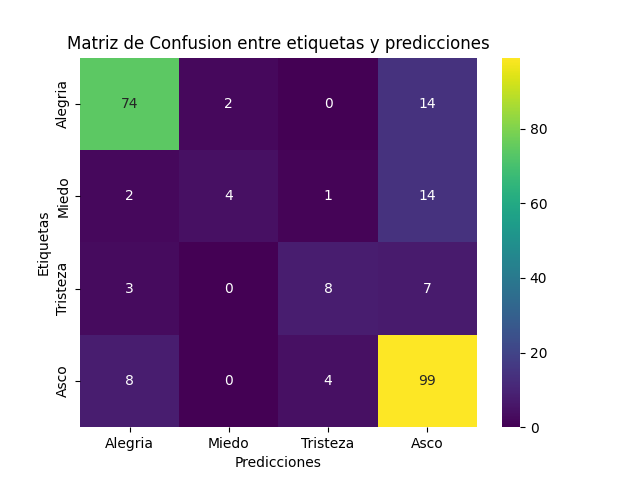
\includegraphics[scale=0.75]{Images & Logos/Results/Matriz_confusion.png} 
	\caption{Matriz de confusión entre etiquetas asignadas y predicciones del algoritmo para el dataset etiquetado}
	\label{figure:Matriz}
\end{figure}


Esta situación se explica en parte porque algunos de estos tweets efectivamente contenían la emoción de miedo junto con asco, pero el modelo solo logró identificar esta ultima, como se ejemplifica en el tweet número 1 en el Cuadro \ref{table:ejemplos_preds}. Esto también ocurrió en el caso de la tristeza, como se aprecia en el tweet número 2. Para la alegría, se observa que también hubo casos en los que tweets fueron etiquetados con esta emoción pero en las predicciones les fue asignado  asco. En muchos casos, esto se debió a que un mismo tweet expresaba dos emociones diferentes, una en cada frase, como se ilustra en el tweet número 3 del cuadro, en donde el autor expresa inicialmente apoyo a una persona y en la siguiente frase rechazo a otra. En relación a los tweets que no tenían etiquetas y, por ende, se representan como neutrales en la Figura \ref{figure:Matriz}, se presentó un fenómeno en el cual los etiquetadores no percibían suficiente carga emocional como para asignar una etiqueta. Sin embargo, el modelo los clasificó con la etiqueta más adecuada según su contenido, como se ilustra en el ejemplo número 4.

\scriptsize
\begin{table}[!htbp]
\scriptsize
\begin{tabular}{{ | p{1.5cm} | p{9cm} | p{1.5cm} | p{1.5cm} | }}
\hline
Numero de Ejemplo & Tweet & Etiquetas & Predicciones \\
\hline
1 & En conclusión \#ElDebateDefinitivo deja claro que Petro es un peligro. Mentiroso, arrogante, tramposo, encubridor, manipulador, violento, pasivo agresivo, resentido. En resumen, una porquería de ser humano, qué digo humano... un demonio.  Petro es el Pol Pot de Ciénaga de Oro & Miedo, Asco & Asco \\
2 & \#ElDebateDefinitivo @sergio\_fajardo  fue a vender ilusiones y convencer no a debatir no propone sólo dice redundancias, me sorprende profe sera que de proyectos no sabe tanto como de licenciatura... & Tristeza, Asco & Asco \\
3 & Juan Roberto Vargas es una persona decente. Néstor Morales es una porquería de persona. \#DebateFinal & Alegria, Asco & Asco \\
4 & \#FedericoEsColombia Me uno Federico Gutiérrez es Colombia. & Neutral & Alegria \\
\hline
\end{tabular}
\caption{Ejemplos de tweets con divergencias entre etiquetas y clasificaciones}
\label{table:ejemplos_preds}
\end{table}

\normalsize







\section{Distribución de emociones por orientación política}


A partir del modelo entrenado se procedió al etiquetado del total del conjunto de datos, es decir los 193,348 tweets relacionados a las elecciones presidenciales en Colombia. El agrupamiento de este etiquetado permite observare  los resultados presentes en la Figura \ref{figure:tweets_total}, donde se muestra el porcentaje de tweets que recibió cada una de las distintas etiquetas emocionales. En dicha figura, se puede observar que la emoción más preponderante fue el asco, abarcando más del 50\% de los tweets. Luego, le sigue la alegría con aproximadamente el 40\%. Por último, tanto la tristeza como el miedo tuvieron una presencia menor, rondando alrededor del 12\% y el 9\%, respectivamente.



\begin{figure}[!htbp]
	\centering
	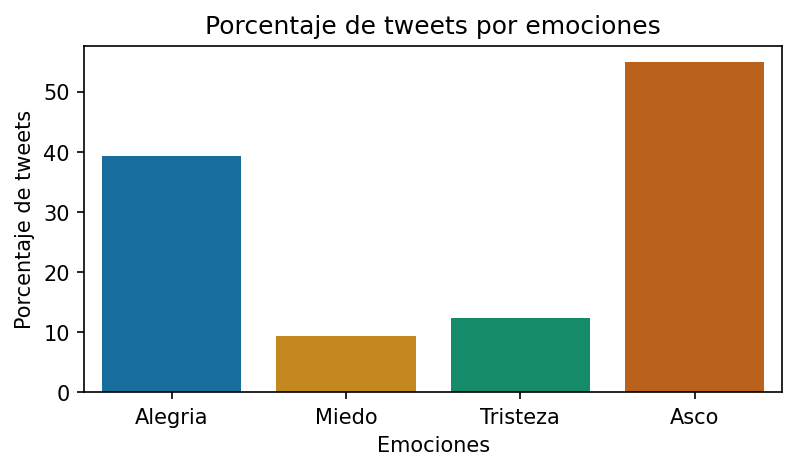
\includegraphics{Images & Logos/Results/Cantidad_de_tweets__por_emocion.png} 
	\caption{Porcentaje de tweets clasificado según emociones por el algoritmo}
	\label{figure:tweets_total}
\end{figure}



Al examinar la distribución de cada emoción según la orientación política asignada al tweet a partir del hashtag empleado, se obtienen los resultados que se presentan en la Figura \ref{figure:porcentaje_emocion}. En este gráfico, se destaca que el sector neutral fue el que mostró una mayor cantidad de tweets etiquetados con miedo, representando aproximadamente el 12\% de sus tweets. Por otro lado, tanto las orientaciones derecha e izquierda tuvieron una presencia menor, alrededor del 8\% y 6\%, respectivamente. En cuanto a la alegría, se revela que los tweets con orientación izquierda asignada, fueron los que presentaron una mayor frecuencia de esta emoción, alcanzando el 58\%. Luego, las orientaciones neutral y derecha tuvieron alrededor de un 30\% cada uno. Respecto al asco, se destaca la preeminencia de los tweets con la orientación de derecha asignada, representando un 69\% del total. La orientación neutral se ubica en segundo lugar con un 60\% de los tweets, mientras que los tweets con la orientación izquierda asignada tienen el menor porcentaje de los tres, un 40\%. Finalmente, en relación a la tristeza, la orientación  neutral fue la que mostró una mayor presencia de esta emoción con un 22\% de su total, cifra significativamente mayor que las orientaciones derecha e izquierda, que tuvieron un 6\% y 3\%, respectivamente.



\begin{figure}[!htbp]
	\centering
	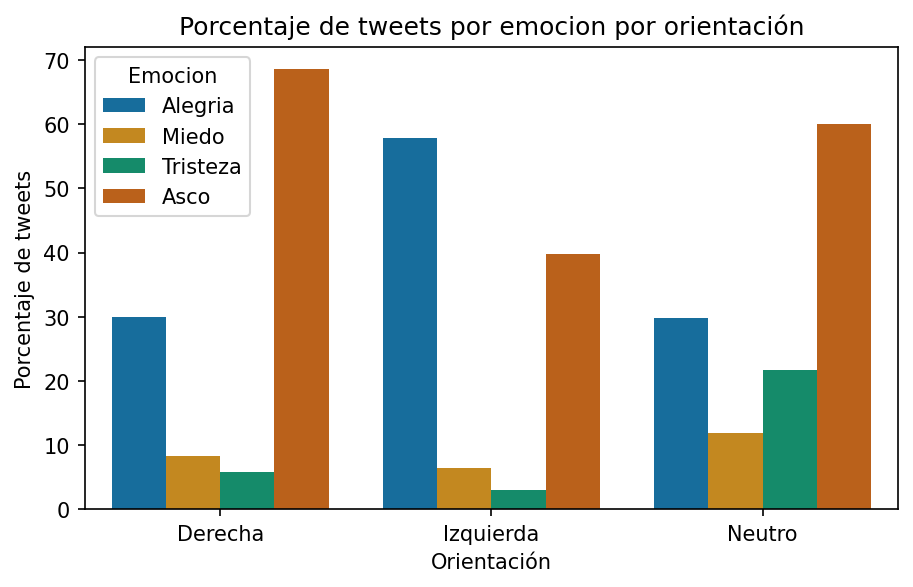
\includegraphics{Images & Logos/Results/Porcentaje de tweets por emocion por sector.png}
	\caption{Porcentaje de tweets clasificados según emoción por el algoritmo, separado por orientación política del hashtag}
	\label{figure:porcentaje_emocion}
\end{figure}





\section{Emociones a lo largo del tiempo}



En la Figura \ref{figure:tweets_percent_tiempo}, que muestra el porcentaje de tweets que tuvo cada emoción en un día especifico, se puede observar que el 29 de mayo fue un día particularmente activo en términos emocionales. Durante ese día, alrededor del 27\% de los tweets estuvieron asociados con las emociones de alegría y miedo, un 20\% con tristeza y un 9\% con asco. Este día coincidió con la primera vuelta presidencial. De manera similar, entre los días 9 y 10 de junio hubo un repunte en las emociones de asco, tristeza y miedo, con porcentajes del 9\%, 6\% y 5\% respectivamente. Estos días estuvieron marcados por el evento conocido como Petro videos, que se refiere a la filtración de videos grabados durante una reunión del equipo del candidato Petro, en la que se discutían estrategias de campaña\footnote{\url{https://es.wikipedia.org/wiki/Petrovideos}}. Posteriormente, se observa otro aumento en las emociones de asco, miedo y tristeza alrededor del 16 de junio, fecha en la que se habló del debate final al cual el candidato Rodolfo Hernández se negó a participar. Finalmente, el 19 de junio, que corresponde a la segunda vuelta, se observa un incremento en las emociones de alegría, tristeza y miedo.

\begin{figure}[!htbp]
	\centering
	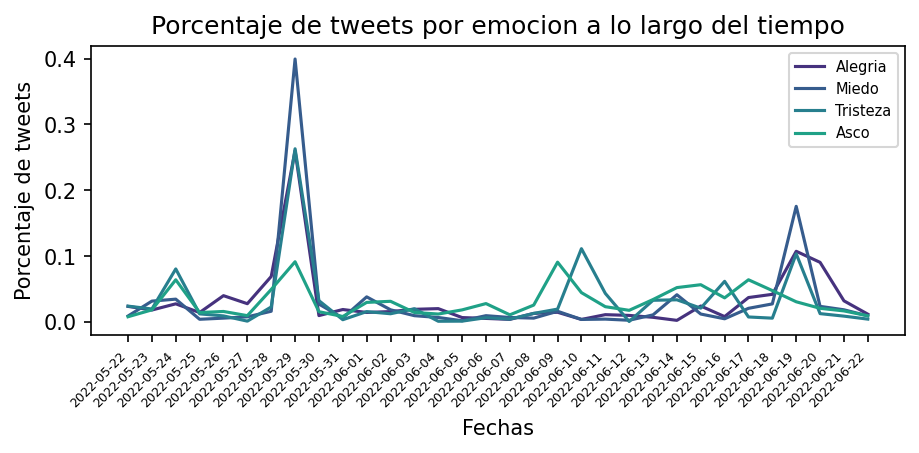
\includegraphics{Images & Logos/Results/Porcentaje de tweets por emocion a lo largo del tiempo.png}
	\caption{Porcentaje diario del total de tweets clasificados en cada emoción a lo largo del tiempo}
	\label{figure:tweets_percent_tiempo}
\end{figure}

En relación a cada emoción y orientación, se obtuvo el porcentaje correspondiente que tuvieron los tweets asignados a cada orientación en un día particular. Esto se logró dividiendo el número de tweets de una orientación, con una emoción específica en dicho día entre el total de tweets de esa misma orientación con esa misma emoción. Esto se puede apreciar en la Figura \ref{figure:tweets_percent_alegria_tiempo} para la emoción de alegría, en la cual se observa que el 29 de mayo todas las orientaciones  experimentaron un repunte en esta emoción. Posteriormente, cerca del 19 de junio, día de la segunda vuelta de las elecciones, las tres orientaciones muestran un crecimiento en la emoción de alegría, que luego disminuye, primero en la derecha, seguida por la orientación neutral y finalmente en la izquierda.




\begin{figure}[!htbp]
	\centering
	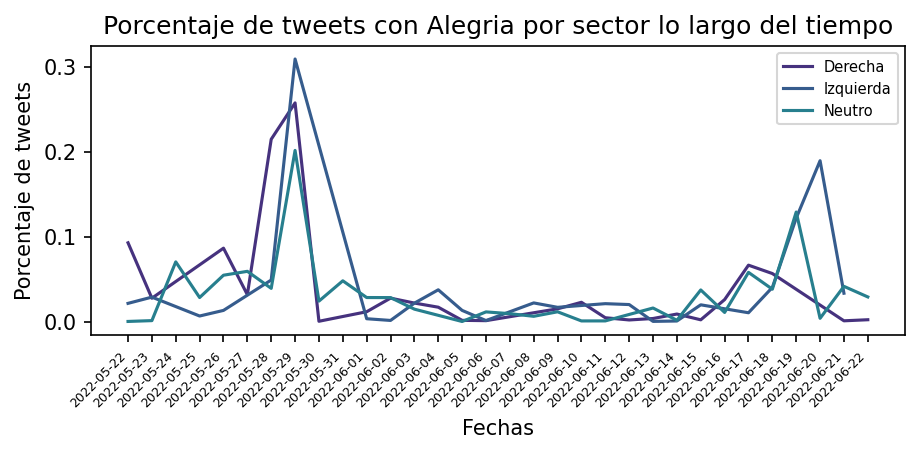
\includegraphics{Images & Logos/Results/Porcentaje de tweets con Alegria por sector lo largo del tiempo.png} 
	\caption{Porcentaje diario del total de tweets clasificados como Alegría, para cada orientación política}
	\label{figure:tweets_percent_alegria_tiempo}
\end{figure}


En el caso del miedo, se puede observar en la Figura \ref{figure:tweets_percent_Miedo_tiempo} un notable pico en las tres orientaciones entre el 29 de mayo y el 1 de junio, como respuesta a la primera vuelta. Posteriormente, el 9 de junio hubo un repunte del miedo en la derecha, como consecuencia del fenómeno conocido como los "Petro videos". El 14 de junio también se evidencia un aumento en el miedo en la derecha, debido a rumores de un posible estallido social. Finalmente, cerca del 19 de junio se observa un pico de miedo en las orientaciones neutro e izquierda.

\begin{figure}[!htbp]
	\centering
	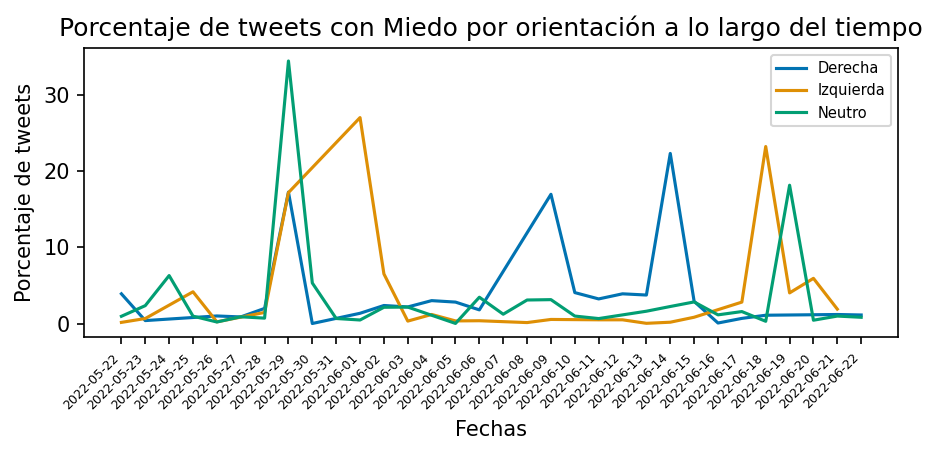
\includegraphics{Images & Logos/Results/Porcentaje de tweets con Miedo por sector lo largo del tiempo.png}
	\caption{Porcentaje diario del total de tweets clasificados como Miedo, para cada orientación política}
	\label{figure:tweets_percent_Miedo_tiempo}
\end{figure}

En cuanto a la tristeza, se aprecia en la Figura \ref{figure:tweets_percent_Tristeza_tiempo} que las tres orientaciones tuvieron un repunte inicial cerca del 24 de mayo, como resultado de un debate. Entre el 29 de mayo y el 1 de junio, la izquierda y la orientación neutral experimentaron otro incremento, alcanzando un 36\% y un 22\% respectivamente. El 9 de junio se observa un aumento en la tristeza en la derecha, relacionado con los "Petro videos", y el 10 de junio hubo un repunte en la orientación neutral, en el que se discutieron temas decepcionantes relacionados con las elecciones. El 14 de junio, la derecha experimentó nuevamente un aumento en la tristeza, también relacionado con la posibilidad de un estallido social. Finalmente, cerca del 19 de junio, todos los sectores mostraron un incremento en la tristeza.

\begin{figure}[!htbp]
	\centering
	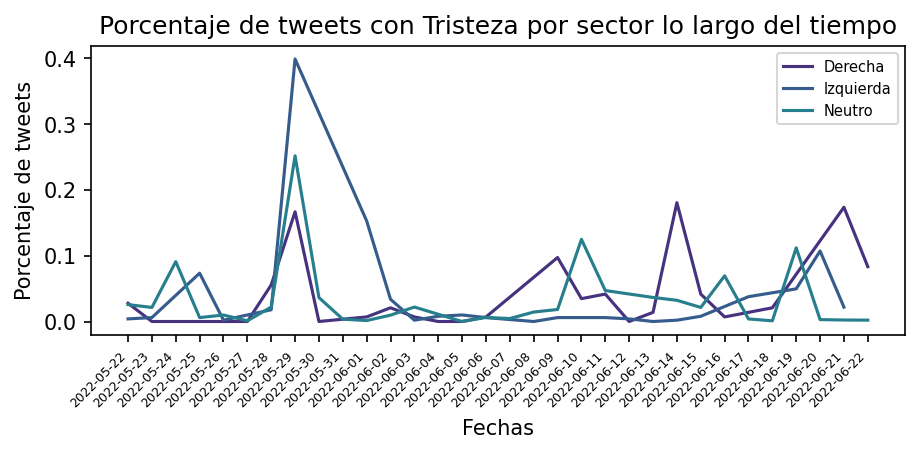
\includegraphics{Images & Logos/Results/Porcentaje de tweets con Tristeza por sector lo largo del tiempo.png}
	\caption{Porcentaje diario del total de tweets clasificados como Tristeza, para cada orientación política}
	\label{figure:tweets_percent_Tristeza_tiempo}
\end{figure}

En relación al asco, se puede observar en la Figura \ref{figure:tweets_percent_Asco_tiempo} que al inicio hay un pico en la orientación neutral el 24 de mayo, como reacción al debate. Luego, todos las orientaciones experimentaron un repunte el 29 de mayo. Es notable el gran pico que tuvo la derecha el 9 de junio, coincidiendo con los "Petro videos", con más del 27\%. De manera similar, la izquierda alcanzó su punto máximo el 17 de junio, llegando a cerca del 20\%. En esta fecha se habló de la negativa del candidato Rodolfo Hernández a participar en el debate final.

\begin{figure}[!htbp]
	\centering
	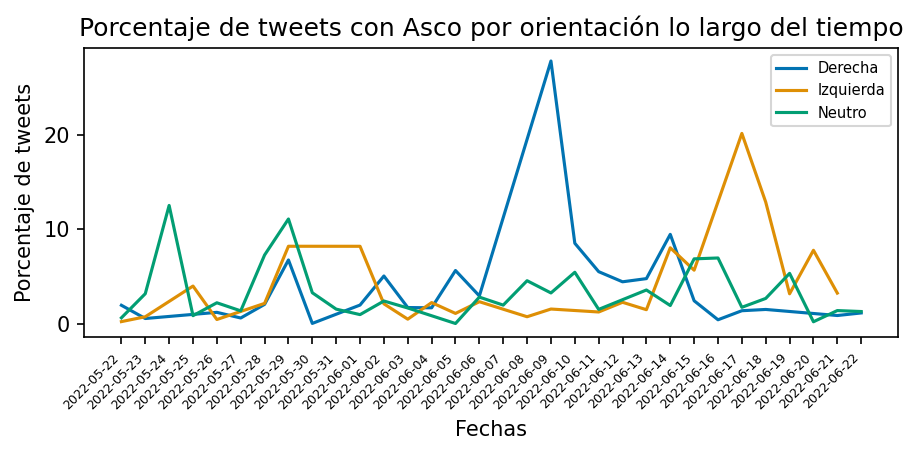
\includegraphics{Images & Logos/Results/Porcentaje de tweets con Asco por sector lo largo del tiempo.png} 
	\caption{Porcentaje diario del total de tweets clasificados como Asco, para cada orientación política}
	\label{figure:tweets_percent_Asco_tiempo}
\end{figure}














